\documentclass[12pt]{article}
\usepackage[margin=1.5cm]{geometry}
\usepackage{amsmath}
\usepackage{graphicx}
\title{RC Circuits Lab: Electronic Filters}

\begin{document}
\maketitle

\section{An Essential Math Tool}

The Fourier transform of a function $f(t)$ is defined as:

\begin{equation}
\mathcal{F}(f(t)) = \tilde{F}(\omega) = \int_{-\infty}^{\infty} f(t) e^{-j\omega t} dt
\label{eq:eq1}
\end{equation}

In Eq. \ref{eq:eq1}, $\omega$ is the angular frequency, measured in radians per unit time.  Let $f(t) = g'(t)$.  Substituting into Eq. \ref{eq:eq1}, and integrating by parts, we have

\begin{equation}
\tilde{F}(\omega) = g(t) e^{-j\omega t} |_{-\infty}^{\infty} + j\omega \int_{\infty}^{-\infty} g(t)  e^{-j\omega t} dt
\label{eq:eq2}
\end{equation}

For physical signals that represent finite energy, $\lim_{|t|\rightarrow\infty} g(t) = 0$.  This requirement simplifies Eq. \ref{eq:eq2} by making the first term on the right-hand side vanish.  We have

\begin{equation}
\tilde{F}(\omega) = j\omega \int_{\infty}^{-\infty} g(t)  e^{-j\omega t} dt = j\omega\mathcal{F}(g(t))
\end{equation}

The result may be summarized:

\begin{equation}
\boxed{
\mathcal{F}(g'(t)) = j\omega\mathcal{F}(g(t))
}
\end{equation}

One utility of this result is that differential equations in the time-domain may be converted to algebraic equations in the Fourier domain, making them easier to apply.

\section{Two Simple Circuits}

\begin{figure}
\centering
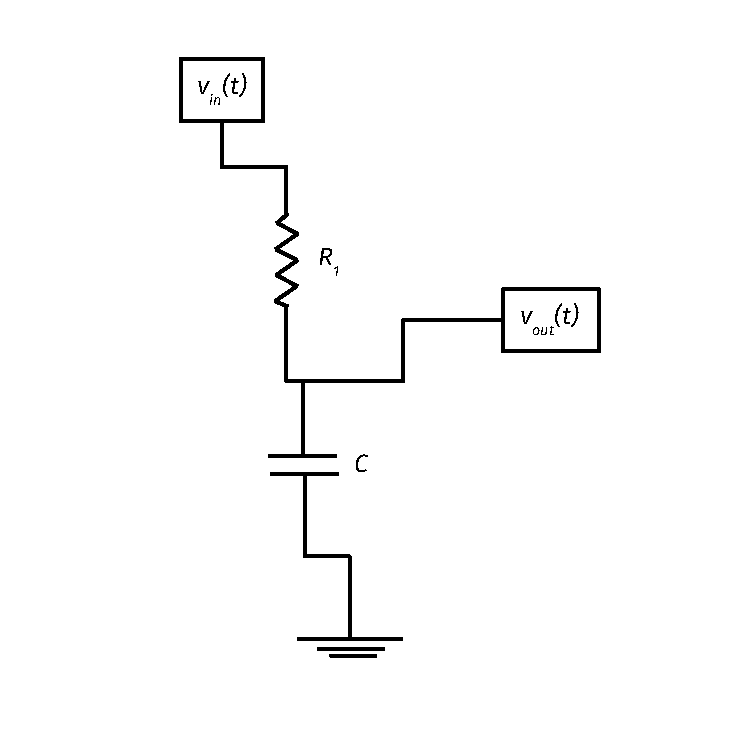
\includegraphics[width=0.35\textwidth,trim=0cm 1cm 0cm 0cm,clip=true]{LowPass.pdf}
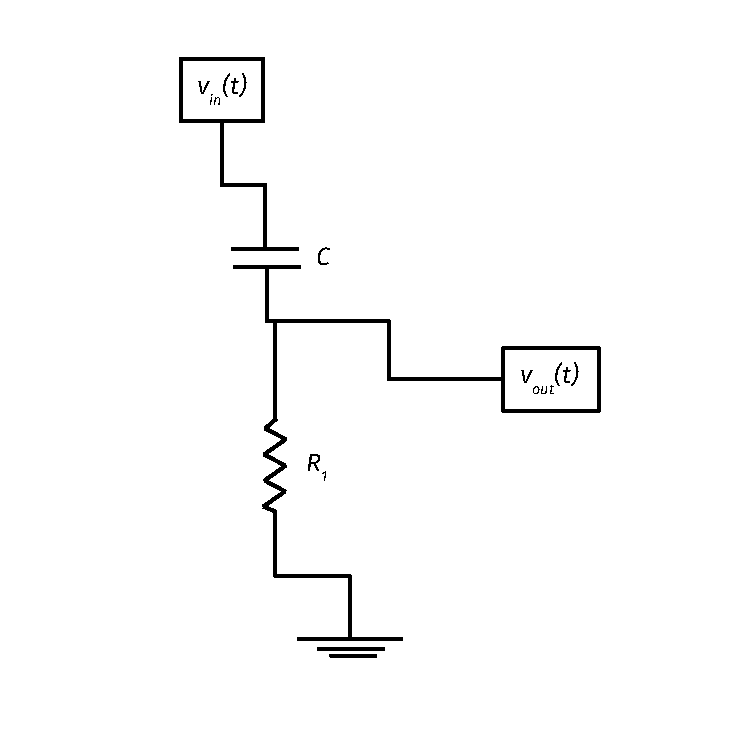
\includegraphics[width=0.35\textwidth,trim=0cm 1cm 0cm 0cm,clip=true]{HighPass.pdf}
\caption{\label{fig:fig2} (Left) A single-pole RC low-pass filter. (Right) A single-pole RC high-pass filter.}
\end{figure}

A simple RC circuit is shown in Fig. \ref{fig:fig2}.  The resistance $R$ is given, and the capacitance $C$ is the ratio of the charge stored on the capacitor, $q$, to the voltage required to place that charge on the capacitor, $V$:

\begin{align}
q &= CV \\
i(t) &= C \frac{dV}{dt} \\
\tilde{i}(\omega) &= j\omega C \tilde{V}(\omega) \\
\frac{\tilde{V}(\omega)}{\tilde{i}(\omega)} &= \frac{1}{j\omega C}
\end{align}

Thus, Ohm's law says that the frequency-dependent resistance, or \textit{impedance}, of a capacitor is

\begin{equation}
\boxed{
Z_C = \frac{1}{j\omega C}
}
\label{eq:eq5}
\end{equation}

The \textbf{transfer function} of the RC circuit in Fig. \ref{fig:fig2} is the ratio of the output voltage to the input voltage, as with a voltage divider.  However, the derivation of this ratio produces

\begin{equation}
\frac{\tilde{v}_{out}(\omega)}{\tilde{v}_{in}(\omega)} = \frac{\frac{1}{j\omega C}}{R+\frac{1}{j\omega C}} = \frac{1}{j\omega R C + 1}
\label{eq:trans2}
\end{equation}

Let the \textit{time-constant} be defined as $\tau = RC$, and $\omega_0 = 1/\tau$.  Equation \ref{eq:trans2} may be written:

\begin{equation}
\frac{\tilde{v}_{out}(\omega)}{\tilde{v}_{in}(\omega)} = -\frac{j\omega_0}{\omega - j\omega_0}
\label{eq:eq6}
\end{equation}

The magnitude and phase of Eq. \ref{eq:eq6} are

\begin{align}
M_{LP}(\omega) &= \left( 1 + \left( \frac{\omega}{\omega_0}\right)^2 \right)^{-1/2} \\
\phi_{LP}(\omega) &= -\tan^{-1}\left(\frac{\omega}{\omega_0}\right)
\label{eq:eq7}
\end{align}

The low-pass transfer function $M_{LP}(\omega)$ attenuates frequencies much larger than $\omega_0$, and the $\phi_{LP}(\omega)$ function shows that there is a frequency-dependent phase-shift.  The high-pass filter in Fig. \ref{fig:fig2} (right) is similar to the low-pass filter in Fig. \ref{fig:fig2} (left).  Following the same arguments as the low-pass case, the complex transfer function is

\begin{equation}
\frac{\tilde{v}_{out}(\omega)}{\tilde{v}_{in}(\omega)} = \frac{\omega}{\omega - j\omega_0}
\label{eq:trans3}
\end{equation}

The magnitude and phase of Eq. \ref{eq:trans3} are

\begin{align}
M_{HP}(\omega) &= \left( 1 + \left( \frac{\omega_0}{\omega}\right)^2 \right)^{-1/2} \\
\phi_{HP}(\omega) &= \tan^{-1}\left(\frac{\omega_0}{\omega}\right)
\end{align}

Unlike the voltage divider, the circuits in Fig. \ref{fig:fig2} have capacitors.  The filtering in these cases is driven by how quickly these capacitors can be charged and discharged, regardless of where they are in the circuit.

\section{Building a Passive Differentiator}

Consider a single-pole high pass filter, with transfer function given by Eq. \ref{eq:trans3}.  Choose a value for $\omega_0$ much larger than any frequency in the expected input signal: $\omega_0 \gg \omega$.  The transfer function is approximately:

\begin{equation}
\frac{\tilde{v}_{out}(\omega)}{\tilde{v}_{in}(\omega)} \approx \frac{\omega}{-j\omega_0} = j\omega \tau = j\omega RC
\label{eq:eq19}
\end{equation}

Rearranging Eq. \ref{eq:eq19}, and switching back to the time-domain:

\begin{align}
\tilde{v}_{out}(\omega) &\approx j\omega \tau \tilde{v}_{in}(\omega) \\
v_{out}(t) &\approx \tau \frac{dv_{in}}{dt}
\label{eq:eq20}
\end{align}

Equation \ref{eq:eq20} shows that with the correct choice of resistance and capacitance, the circuit output is the derivative of the input, with a \textit{gain} equal to $\tau = RC$.  This circuit is known as a \textit{passive differentiator}.

\section{Building a Passive Integrator}

Consider a single-pole low-pass filter, with transfer function given by Eq. \ref{eq:trans2}.  Choose a value for $\omega_0$ much smaller than any frequency in the expected input signal: $\omega_0 \ll \omega$.  The transfer function is approximately:

\begin{equation}
\frac{\tilde{v}_{out}(\omega)}{\tilde{v}_{in}(\omega)} \approx \frac{-j\omega_0}{\omega}
\label{eq:eq21}
\end{equation}

Rearranging Eq. \ref{eq:eq21}, switching back to the time-domain, and integrating both sides:

\begin{align}
j\omega \tilde{v}_{out}(\omega) &\approx \omega_0 \tilde{v}_{in}(\omega) \\
\frac{dv_{out}}{dt} &= \omega_0 v_{in}(t) \\
v_{out}(t) &= \frac{1}{RC} \int_{t_1}^{t_2} v_{in}(t) dt
\label{eq:eq22}
\end{align}

Equation \ref{eq:eq22} shows that with the correct choice of resistance and capacitance, the circuit output is the integral of the input between two set times, with a \textit{gain} equal to $1/RC$.  This circuit is known as a \textit{passive integrator}.

\section{Summary of Passive Differentiator and Integrator}

\begin{itemize}
\item By choosing a large value of $RC$, relative to input frequencies, the output of a single-pole high-pass filter is proportional to the derivative of the input, with gain $RC$.
\item By choosing a small value of $RC$, relative to input frequencies, the output of a single-pole low-pass filter is proportional to the integral of the input, with gain $1/RC$.
\end{itemize}

\end{document}